\documentclass{beamer}
\usepackage[version=4]{mhchem} 
\usepackage{tikz}


\usetheme{Madrid}
\usecolortheme{beaver}

\title{Unit 2}
\subtitle{Ondas}
\author{Mr. Maxwell}
\institute{PACS}
\date{\today}


\begin{document}

\frame{\titlepage}
\frame{\tableofcontents}

\section{Vocabulario de ondas}

\subsection{Tipos de olas}

\subsubsection{ondas mecánicas}

\begin{frame}
    \frametitle{ondas mecánicas}
    
    \begin{enumerate}
        \item requiere un medio o material (es decir, gas, líquido, sólido) para la transmisión
        \item la energía proviene de una fuente vibratoria
        \item la onda pasa a través de un medio, pero el medio en sí no viaja junto con la onda a medida que se transmite energía.
    \end{enumerate}
\end{frame}

\subsubsection{ondas electromagnéticas}

\begin{frame}
    \frametitle{ondas electromagnéticas}
    
    \begin{enumerate}
        \item no necesita un medio
        Entre ellos se incluyen la luz visible, así como la luz infrarroja y ultravioleta, las microondas, los rayos X y los rayos gamma.
        \item Estas ondas son generadas por oscilaciones de campos eléctricos y magnéticos de partículas cargadas.
        \item Todas las ondas electromagnéticas en el vacío se mueven a la misma velocidad. Esta velocidad, 3 × 108 m/s, se conoce como velocidad de la luz y está representada por la letra c.
    \end{enumerate}
\end{frame}

\subsection{Propiedades de onda}

\subsubsection{amplitud}

\begin{frame}
    \frametitle{amplitud}
    
\pause La distancia desde una línea media hasta una cresta o valle
    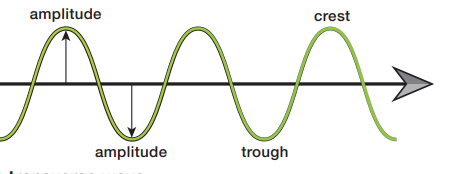
\includegraphics[width=9cm]{../../../../public/amplitude.png}
\end{frame}

\subsubsection{longitud de onda}

\begin{frame}
    \frametitle{longitud de onda}
    \pause La distancia de una cresta o valle a la siguiente.
    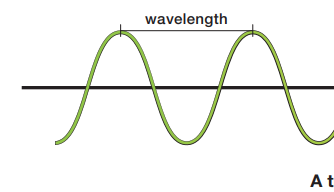
\includegraphics[width=9cm]{../../../../public/wavelength.png}
\end{frame}

\subsubsection{frecuencia}

\begin{frame}
    \frametitle{frecuencia}
    \pause  El número de longitudes de onda que pasan por un punto en un período de tiempo determinado (generalmente un segundo) es la frecuencia de la onda (f).
    \vspace{1cm}
    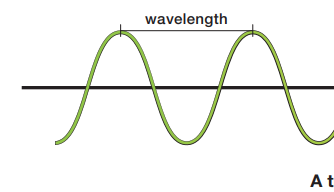
\includegraphics[width=8cm]{../../../../public/wavelength.png}
\end{frame}




\subsubsection{velocity}

\end{document}